\tikzset{
	treenode/.style = {shape=rectangle, rounded corners,
		draw, align=center,
		top color=white, bottom color=blue!20},
	root/.style     = {treenode, font=\ttfamily\normalsize, bottom color=red!30},
	env/.style      = {treenode, font=\ttfamily\normalsize},
	dummy/.style    = {circle,draw},
	level 1/.style={sibling distance=6cm, level distance = 3em},
	level 2/.style={sibling distance=2.5cm,level distance = 5em}, 
	level 3/.style={sibling distance=2cm},
	blueRed/.style={env, top color=blue, bottom color=red} 
}
%\begin{document}
	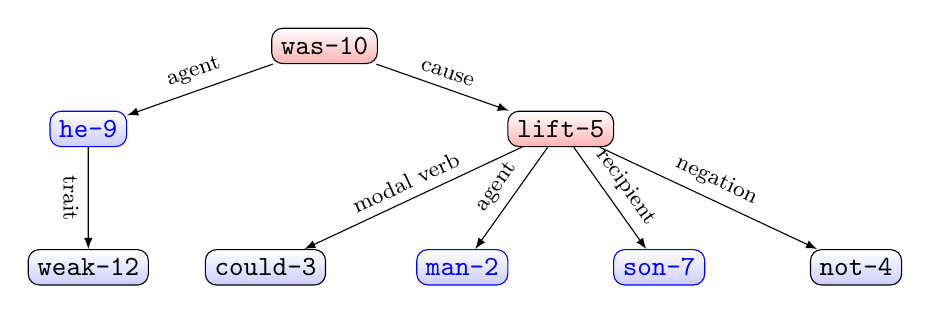
\begin{tikzpicture}
	[
	grow                    = down,
	sibling distance        = 50em,
	level distance          = 5em,
	edge from parent/.style = {draw, -latex},
	every node/.style       = {font=\footnotesize},
	sloped
	]
	\node [root] {was-10}
	child { node [env, blue] {he-9}
	  child {node [env] {weak-12}
			edge from parent node [below] {trait} }
	   edge from parent node [above] {agent}}
	child { node [env, bottom color=red!30] {lift-5} 
	  child {node [env]  {could-3}
	  	edge from parent node [above] {modal verb} }	
	  child {node [env, blue]  {man-2}
	  	edge from parent node [above] {agent} }
	  child {node [env, blue]  {son-7}
	  	edge from parent node [above] {recipient}}
	  child {node [env]  {not-4}
			edge from parent node [above] {negation} }
		edge from parent node [above] {cause}};
	
	\end{tikzpicture}